\documentclass[a4paper, 12pt]{article}
\usepackage[a4paper, top = 1.5cm, bottom = 1.5cm, left = 1cm, right = 1cm]{geometry}
\usepackage{graphicx}
\usepackage{subcaption}
\usepackage{mathtools}
\usepackage{amsfonts}
\usepackage{longtable}
\usepackage{float}
\usepackage[english, russian]{babel}
\title{Лабораторная работа № 3.5.1-3.5.2 "Изучение плазмы газового разряда в неоне"}
\author{Кирилл Шевцов Б03-402}
\date{16.09.2025}
\begin{document}
\maketitle
\section*{Цель работы}
Изучить вольт-амперную характеристику тлеющего разряда, изучить свойства плазмы методом зондовых
характеристик.
\section*{Оборудование}
Стеклянная газоразрядная трубка, наполненная неоном, источник напряжения, делитель напряжения, потенциометр,
амперметр, вольтметры, амперметры, переключатели.
\section*{Лабораторные установки}
Стеклянная газоразрядная трубка имеет ненагреваемый полый катод, три анода и геттерный узел - стеклянный баллон,
на внутреннюю поверхность которого напылена газопоглощающая плёнка (геттер). Трубка наполнена изотопом неона при давлении
2 мм. рт. столба. Катод и один из анодов (первый или второй) с помощью переключателя $P_{1}$ подключаются через балластный резистор
$R_{b}$ к регулируемому ВИП.
\begin{figure}[htbp]
    \centering
    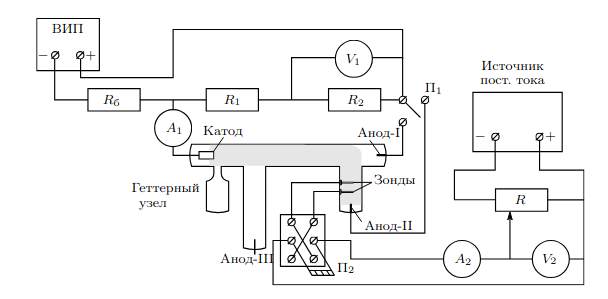
\includegraphics[width=1.0\linewidth]{p1.png}
    \caption{установка для исследования газового разряда}
    \label{установка для исследования газового разряда}
\end{figure}\\
При подключении первого анода к ВИП, между ним и катодом возникает газовый разряд. Ток разряда измеряется
амперметром $A_{1}$, падение напряжения - на вольтметре $V_{1}$, подключенным к трубке через делитель напряжения с
коэффициентом, равным $\alpha = \frac{R_{1} + R_{2}}{R_{2}}$. При подключении к ВИП второго анода, возникает газовый разряд между
катодами и вторым анодом, где находится двойной зонд, необходимый для диагностики плазмы. Третий анод в работе не используется.
\section*{Выполнение работы}
\begin{enumerate}
    \item Настроим установку для ВАХ газового разряда согласно инструкции, плавно увеличивая показания ВИП, запишем напряжение
    зажигания, показание вольтметра $V_{1}$:
    \begin{equation}
        U_{0} = 152.52\pm 0.01\ \text{В}
    \end{equation}
    \item С помощью вольтметра $V_{1}$ и амперметра $A_{1}$ измерим ВАХ газового разряда $I_{p}(U_{p})$. Ток изменяется в диапазоне $0.5 - 5.0$ мА.
    \begin{table}[htbp]
        \centering
        \begin{tabular}{|c|c|c|c|c|c|c|c|c|c|}
            \hline
            $I_{p}\uparrow$, мА & 0.543 & 0.730 & 1.143 & 1.479 & 1.800 & 2.105 & 2.520 & 2.837 & -\\ \hline
            $U_{p}$, В & 26.89 & 26.51 & 26.30 & 26.35 & 26. 40 & 26.48 & 26.55 & 26.62 & -\\ \hline
            $I_{p}\uparrow$, мА & 3.128 & 3.524 & 3.829 & 4.150 & 4.477 & 4.727 & 5.050 & \multicolumn{2}{|c|}{-}\\ \hline
            $U_{p}$, В & 26.67 & 26.72 & 26.75 & 26.77 & 26.79 & 26.80 & 26.81 & \multicolumn{2}{|c|}{-}\\ \hline
            $I_{p}\downarrow$, мА & 4.790 & 4.417 & 4.055 & 3.788 & 3.472 & 3.162 & 2.873 & 2.503 & 2.165\\ \hline
            $U_{p}$, В & 26.80 & 26.78 & 26.76 & 26.74 & 26.71 & 26.66 & 26.61 & 26.54 & 26.47\\ \hline
            $I_{p}\downarrow$, мА & 1.803 & 1.507 & 1.197 & 0.817 & 0.665 & 0.538 & \multicolumn{3}{|c|}{-}\\ \hline
            $U_{p}$, В & 16.41 & 26.35 & 26.31 & 26.41 & 26.65 & 26.90 & \multicolumn{3}{|c|}{-}\\
            \hline
        \end{tabular}
    \end{table}
    \item Построим ВАХ разряда в координатной сетке. По наклону кривой определим максимальное дифференциальное сопротивление $R_{dif} = \frac{dU}{dI}$.
    \begin{figure}[htbp]
        \centering
        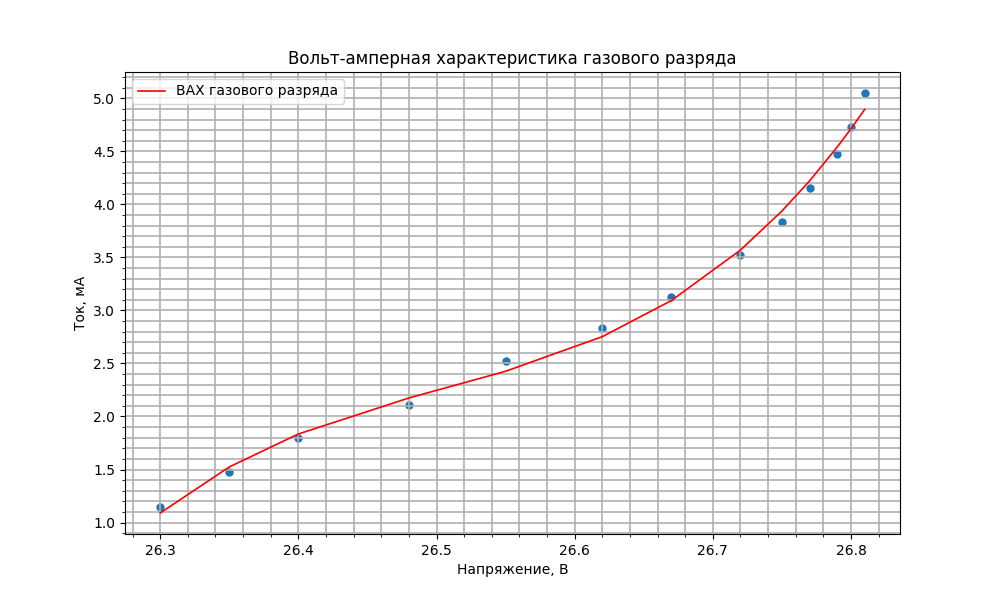
\includegraphics[width=0.9\linewidth]{vax.png}
    \end{figure}
    \item Подготовим установку для анализа зондовой характеристики разряда. Измерим ВАХ двойного зонда, плавно увеличивая напряжение
    от $-U_{0}$ до $U_{0}$ при фиксированном токе разряда $I_{p}$.
    \begin{table}[htbp]
        \centering
        \begin{tabular}{|c|c|c|c|c|c|c|c|c|c|c|c|}
            \hline
            $I_{p}$, мА & \multicolumn{11}{|c|}{$5.000\pm 0.001$}\\ \hline
            $I_{z}\downarrow$, мА & 22.98 & 22.10 & 21.17 & 20.25 & 19.26 & 18.17 & 17.25 & 15.88 & 12.90 & 6.89 & 0.07\\ \hline
            $U_{z}$, В & 24.99 & 22.07 & 19.02 & 16.11 & 13.08 & 10.11 & 8.09 & 6.08 & 4.03 & 2.06 & 0.55\\ \hline
            $I_{z}\uparrow$, мА & -2.66 & -6.74 & -12.96 & -15.90 & -17.13 & -18.19 & -19.38 & -20.37 & -21.34 & -22.33 & -23.18\\ \hline
            $U_{z}$, В & 0.00 & 2.02 & 4.07 & 6.20 & 8.08 & 10.13 & 13.04 & 16.04 & 19.08 & 22.19 & 24.99\\ \hline
            $I_{p}$, мА & \multicolumn{11}{|c|}{$4.005\pm 0.001$}\\ \hline
            $I_{z}\downarrow$, мА & 19.67 & 18.97 & 18.12 & 17.35 & 16.50 & 15.54 & 14.70 & 13.42 & 10.85 & 5.61 & 0.12\\ \hline
            $U_{z}$, В & 24.99 & 22.11 & 19.09 & 16.12 & 13.09 & 10.07 & 8.01 & 6.01 & 4.08 & 2.08 & 0.60\\ \hline
            $I_{z}\uparrow$, мА & -0.15 & -5.71 & -10.78 & -13.37 & -14.62 & -15.34 & -16.29 & -17.17 & -18.00 & -18.76 & -19.56\\ \hline
            $U_{z}$, В & 0.6 & 2.11 & 4.08 & 6.07 & 8.19 & 10.02 & 13.01 & 16.10 & 19.14 & 22.08 & 25.00\\ \hline
            $I_{p}$, мА & \multicolumn{11}{|c|}{$3.101\pm 0.001$}\\ \hline
            $I_{z}\downarrow$, мА & 15.92 & 15.31 & 14.65 & 14.00 & 13.28 & 12.37 & 11.68 & 10.45 & 8.05 & 3.98 & 0.05\\ \hline
            $U_{z}$, В & 24.99 & 22.02 & 19.09 & 16.22 & 13.12 & 10.12 & 8.10 & 6.03 & 4.04 & 2.07 & 0.58\\ \hline
            $I_{z}\uparrow$, мА & -0.04 & -3.82 & -8.03 & -10.41 & -11.56 & -12.26 & -13.07 & -13.75 & -14.42 & -15.07 & -15.70\\ \hline
            $U_{z}$, В & 0.58 & 2.01 & 4.06 & 6.07 & 8.12 & 10.10 & 13.24 & 16.09 & 19.11 & 22.18 & 24.99\\ \hline
            $I_{p}$, мА & \multicolumn{11}{|c|}{$1.513\pm 0.001$}\\ \hline
            $I_{z}\downarrow$, мА & 9.05 & 8.65 & 8.27 & 7.82 & 7.42 & 6.93 & 6.42 & 5.52 & 4.07 & 1.94 & 0.13\\ \hline
            $U_{z}$, В & 24.99 & 22.01 & 19.06 & 16.04 & 13.09 & 10.12 & 8.09 & 5.97 & 4.02 & 2.11 & 0.56\\ \hline
            $I_{z}\uparrow$, мА & -0.13 & -1.88 & -4.06 & -5.52 & -6.37 & -6.84 & -7.34 & -7.73 & -8.16 & -8.56 & -8.95\\ \hline
            $U_{z}$, В & 0.56 & 2.06 & 4.05 & 6.03 & 8.09 & 10.14 & 13.18 & 16.10 & 19.06 & 22.02 & 24.99\\ \hline
        \end{tabular}
        \caption{зондовая характеристика}
    \end{table}
    \item Построим семейство зондовых характеристик на клеточной сетке.
    \begin{figure}[H]
        \centering
        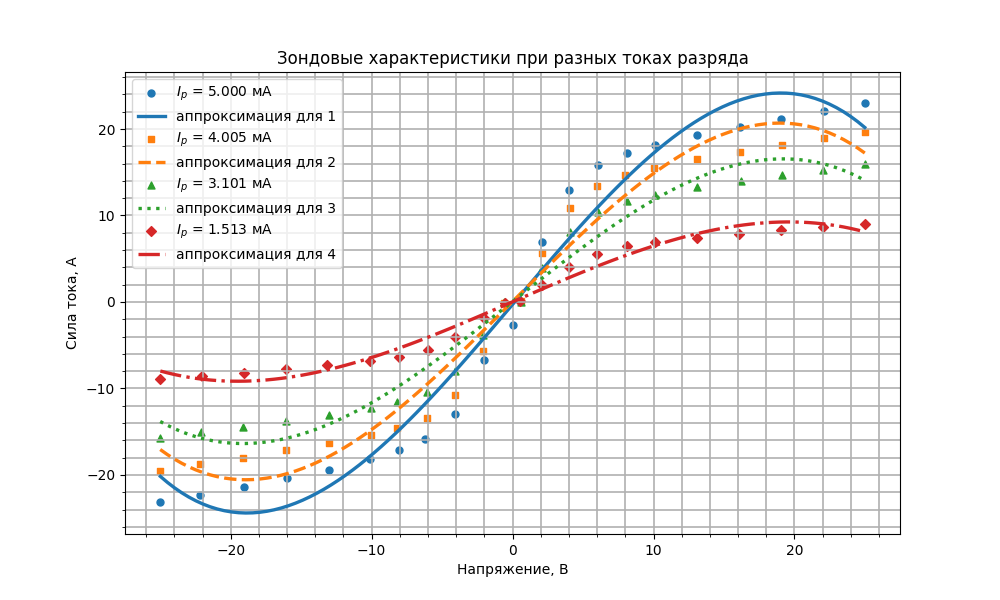
\includegraphics[width=0.9\linewidth]{zond.png}
        \caption{зондовые характеристики для разных токах разряда}
        \label{зондовые характеристики для разных токах разряда}
    \end{figure}
\end{enumerate}
\end{document}